\documentclass[11pt]{article}
\usepackage[margin=1in]{geometry}

% Packages we need
\usepackage{amsmath}
\usepackage{amsfonts}
\usepackage{mathtools}
\usepackage{amsthm}
\usepackage{float}
\usepackage{graphicx}
\usepackage{listings}
\usepackage{color} %red, green, blue, yellow, cyan, magenta, black, white
\usepackage{scrextend}

% Header packages
\usepackage{fancyhdr}
\fancyhf{}
\pagestyle{fancy}

% Algorithms
\usepackage{algorithmic}
\usepackage{algorithm}

% Formatting document
\setcounter{secnumdepth}{0}
\setlength{\parindent}{0in}
\setlength{\parskip}{0.5em}

% Commands
\DeclarePairedDelimiter\ceil{\lceil}{\rceil}
\DeclarePairedDelimiter\floor{\lfloor}{\rfloor}
\newcommand{\ws}{\text{ }}
\newcommand{\e}[1]{\times 10^{#1}}

% Header
\lhead{\textsc{Group 18 Project 2}} % TODO: enter title here
\rhead{
\textsc{Eric Gao -- emg222}\\
\textsc{Yu Su -- ys576}\\
\textsc{Vikram Thapar -- vt87}
} % Authors
\setlength{\headheight}{0.5in}
\cfoot{\thepage}

% Title
\title{Group 18 Project 2} %TODO: enter title here
\author{
  \begin{tabular}{l c l}
    Eric Gao & -- & emg222\\
    Yu Su    & -- & ys576\\
    Vikram Thapar & -- & vt87
  \end{tabular}\\
  \rule{\linewidth}{0.4pt}
}
\date{}


\begin{document}
    \thispagestyle{empty}
    \maketitle

    \section{0 README}
        We have several versions of \texttt{central2d.h}.
        \begin{itemize}
            \item \texttt{central2dBasic.h}: This is the original code.
            \item \texttt{central2d\_handvectorized\_serial.h}: This is the hand vectorized version of the corrector part of the \texttt{compute\_step} function. This code is run serially.
            \item \texttt{central2dParallel.h}: This is the parallelized version with domain decomposition with no vectorization.
            \item \texttt{central2dParallelAligned.h}: This is the parallelized version with \texttt{ivdep}.
            \item \texttt{central2d.h}: This is our fastest version. It is the same as \texttt{central2dParallelAligned.h}.
        \end{itemize}

        You can replace \texttt{central2d.h} with any version you want.

        In the end, we got a speedup of about 5.5 times for a 300 x 300 board with 50 frames when comparing our fastest code with the naive code. In both the naive and our code, we have replaced the \texttt{copysign} function with \texttt{if} statements.

    \section{1 Profiling}
        We began the project with some basic profiling with basic hotspot analysis. We first looked at the vectorization report to see that nothing was vectorized and that could be something we could start with. We then used VTune Amplifier to see where the bottlenecks in the code are.

        The initial report created by VTune Amplifier was:
        \lstinputlisting{table1.txt}

        We see that the slowest part of the code are the two functions: \texttt{limited\_derivs} and \texttt{compute\_step}. Looking at the vectorization report, we see that there is a lot of unvectorized code that could be optimized. Furthermore, there are several parts that are inside of loops that could be parallelized \texttt{omp parallel for} or some other scheme of parallelization.

        We then could use VTune Amplifier to look at specific lines of the code for the given functions and see how long they take. It seems pretty obvious what we need to do for the \texttt{limited\_derivs} function: we need to implement some blocking scheme so that we can do some parallelization using \texttt{OpenMP}. We then saw that the slowest part of the \texttt{compute\_step} function was the corrector step of the function, which took about 3 times as long as the predictor step. The equation that was being implemented involves operations on vectors that could first be vectorized and then parallelized. To do this, we thought we would have to modify how the data was laid out in memory so that it was contiguous in memory.
        
    \section{2 Parallelization}

    \subsection{2.1 Naive omp parallel for}
        We have used  ``pragma loop for" in two functions which are the bottleneck in the calculations: \texttt{limited\_derivs} and \texttt{compute\_step}. The report created by VTune amplifier after modifying the code was:
        \lstinputlisting{table2.txt}
        The above time report shows that the parallelized version of the code for the two bottleneck functions is slower than the basic code. Contradictorily, we found that if we compare the times reported in .o files, the parallel code takes a total time which is approximately 2 times faster than the basic code. We are not able to understand this discrepancy as one would expect similar trends in both the cases.

    \subsection{2.2 Domain decomposition}
        \begin{algorithm}
            \caption{DomainDecomposition()}
            \begin{algorithmic}
                \STATE{Use pragma omp parallel by setting u\_ as the shared variable}
                \STATE{Use omp\_set\_num\_threads(NUM) where NUM is the number of domains. There were 3 ghost cells per domain.}
                \STATE{Initialize vectors in each thread's domain.}
                \STATE{Assign domain index for each thread using omp\_get\_thread\_num().}
                \STATE{Copy the center of domain vectors from u\_ for each thread.}
                \WHILE{time $<$ endTime}
                    \STATE{\texttt{barrier}}
                    \STATE{Serial computation of time step}
                    \STATE{\texttt{barrier}}
                     \STATE{Copy the domain boundary vectors from u\_ for each thread.}
                      \FOR{ i=0; i $<$ 2*Nsteps; i++}
                      \STATE{Here Nsteps is the number of steps by which domain evolves.}
                      \STATE{Flux computation}
                      \STATE{x and y derivatives}
                      \STATE{Predictor and Corrector step}
                      \STATE{Copy back to main grid of the domain}
                      \ENDFOR
                      \STATE{Copy the center domain vectors to u\_}
                      \STATE{\texttt{barrier}}
                \ENDWHILE
            \end{algorithmic}
        \end{algorithm}   
        The serial computation of time step is done on a thread number 0 by using if loop. The alternate/more efficient way is to use pragma omp critical/atomic to perform the serial work. But, we faced some complications while using it as we were not able to synchronize all the threads leading to incorrect results. The number of domains used are N*N where N is an integer.  

        To perform the initial test, we use N = 4, NUM = N*N = 16 on 200by200 system for 50 frames. \textit {Note that for both basic, parallel and later versions, we removed the copysign in minmod and inserted if loops.}  The total time taken by our parallelized code is approximately 0.6 seconds as compared to 1.6 seconds taken by the basic code. So, we were able to obtain the gain of about 2.5 times. Also, when comparing shallow.oParallel and shallow.oBasic, the momentum, volume and range values are approximately equal to each other but not exactly. We believe that this could be due to the machine precision errors as our generated out.mp4 files looks qualitatively the same. Note, that in this code we do not perform any vectorization. So, in the next section, we will go through the vectorization part and  combine it with our parallel code to perform strong and weak scaling.
         
    \section{3 Tuning}

    \subsection{3.1 Initial attempts}
         We tried writing a kernel for the corrector step of the \texttt{compute\_step} function. However, it looked like the most effective thing that we could do was also one of the simplest. We saw that we were always using the \texttt{vec} of length 3 for the innermost loop, so we just unrolled that loop. The compiler then took care of the rest and we went from taking approximately \textbf{4.5e-2} time to about \textbf{3.6e-2}, which is about a 25\% speed up due to this simple optimization.

         We tried another thing which was to try to cache all the \texttt{vec}s that were being used to attempt to increase speed, but it resulted in times similar to the basic approach. We also attempted to implement our own kernel, but it looked like the compiler beat us, since were were getting times comparable to the basic approach. Our attempted kernel is commented out in our \texttt{central2d.h} in the \texttt{compute\_step} function.

    \subsection{3.2 Hand Vectorized Code}
        So afterwards, we went back and we wrote a kernel that works for an 8 x 8 block. This works by looping over all of the relevant \texttt{vec}'s in in the block and loading them into contiguous memory that was \texttt{\_mm\_malloc}'d in the \texttt{Central2D} class. We then wrote about 2000 lines of hand vectorized code to perform the corrector step of the \texttt{compute\_step} function. The relevant code can be found in \texttt{central2d\_handvectorized\_serial.txt}. 

        We then added timers surrounding the corrector step of the \texttt{compute\_step} function. We then ran on the initial 200 x 200 simulation to see the speedup.

        \begin{figure}[H]
            \centering
            \begin{tabular}{c | c}
            Naive times & Hand vectorized times\\
            \hline
            9.019375e-04 & 7.851124e-04 \\
            8.959770e-04 & 7.750988e-04 \\
            9.019375e-04 & 7.801056e-04 \\
            8.959770e-04 & 7.729530e-04 \\
            9.009838e-04 & 7.808208e-04 \\
            8.931160e-04 & 7.739067e-04 \\
            9.021759e-04 & 7.810593e-04 \\
            8.950233e-04 & 7.739067e-04 \\
            9.019375e-04 & 7.879734e-04 \\
            8.950233e-04 & 7.741451e-04
            \end{tabular}
        \end{figure}

        From this we can see that we get about a 15\% speed up, which is not that great considering how much code we wrote and how difficult it was to debug.

        One particular reason why it was not that great of a speedup was because we have to copy data from memory over from unaligned memory into aligned memory and then copy the results back into the appropriate result vectors. One way to overcome this would be to refactor the C++ code to use C style arrays. If we do that, we could call \texttt{\_mm\_malloc} on the arrays initially created. We can then avoid having to reload arrays every time we call our kernel. However, this required extensive refactoring of the C++ code, so we did not do this.

    \subsection{3.3 Vectorization using ivdep}
        To perform vectorization on this code, we have used pragma ivdep. As mentioned in intel website, ivdep provides the instruction to the compiler to ignore vector dependecies and performs the auto vectorization.  In the profiling section, we show that the limited\_derivs is the computationally expensive step. So we decided to put \#pragma omp ivdep in limdiff function in central2d.h. The modified function looks like

        \begin{lstlisting}
static void limdiff(vec& du, const vec& um, const vec& u0, const vec& up) {
    #pragma ivdep
    for (int m = 0; m < du.size(); ++m)
        du[m] = Limiter::limdiff(um[m], u0[m], up[m]);
}
        \end{lstlisting}
        On adding ivdep, we were able to get a significant gain. The parallelized code run for section 2.2 now takes a total time of 0.43 seconds. 
   
    \section{4 Scaling}
        We split the scaling section into two subsections. For the scaling, we use our fastest code which is the parallelized code combined with the vectorization of limdiff using ivdep.
             
    \subsection{4.1 Strong Scaling}
        \begin{figure}[H]
            \centering
            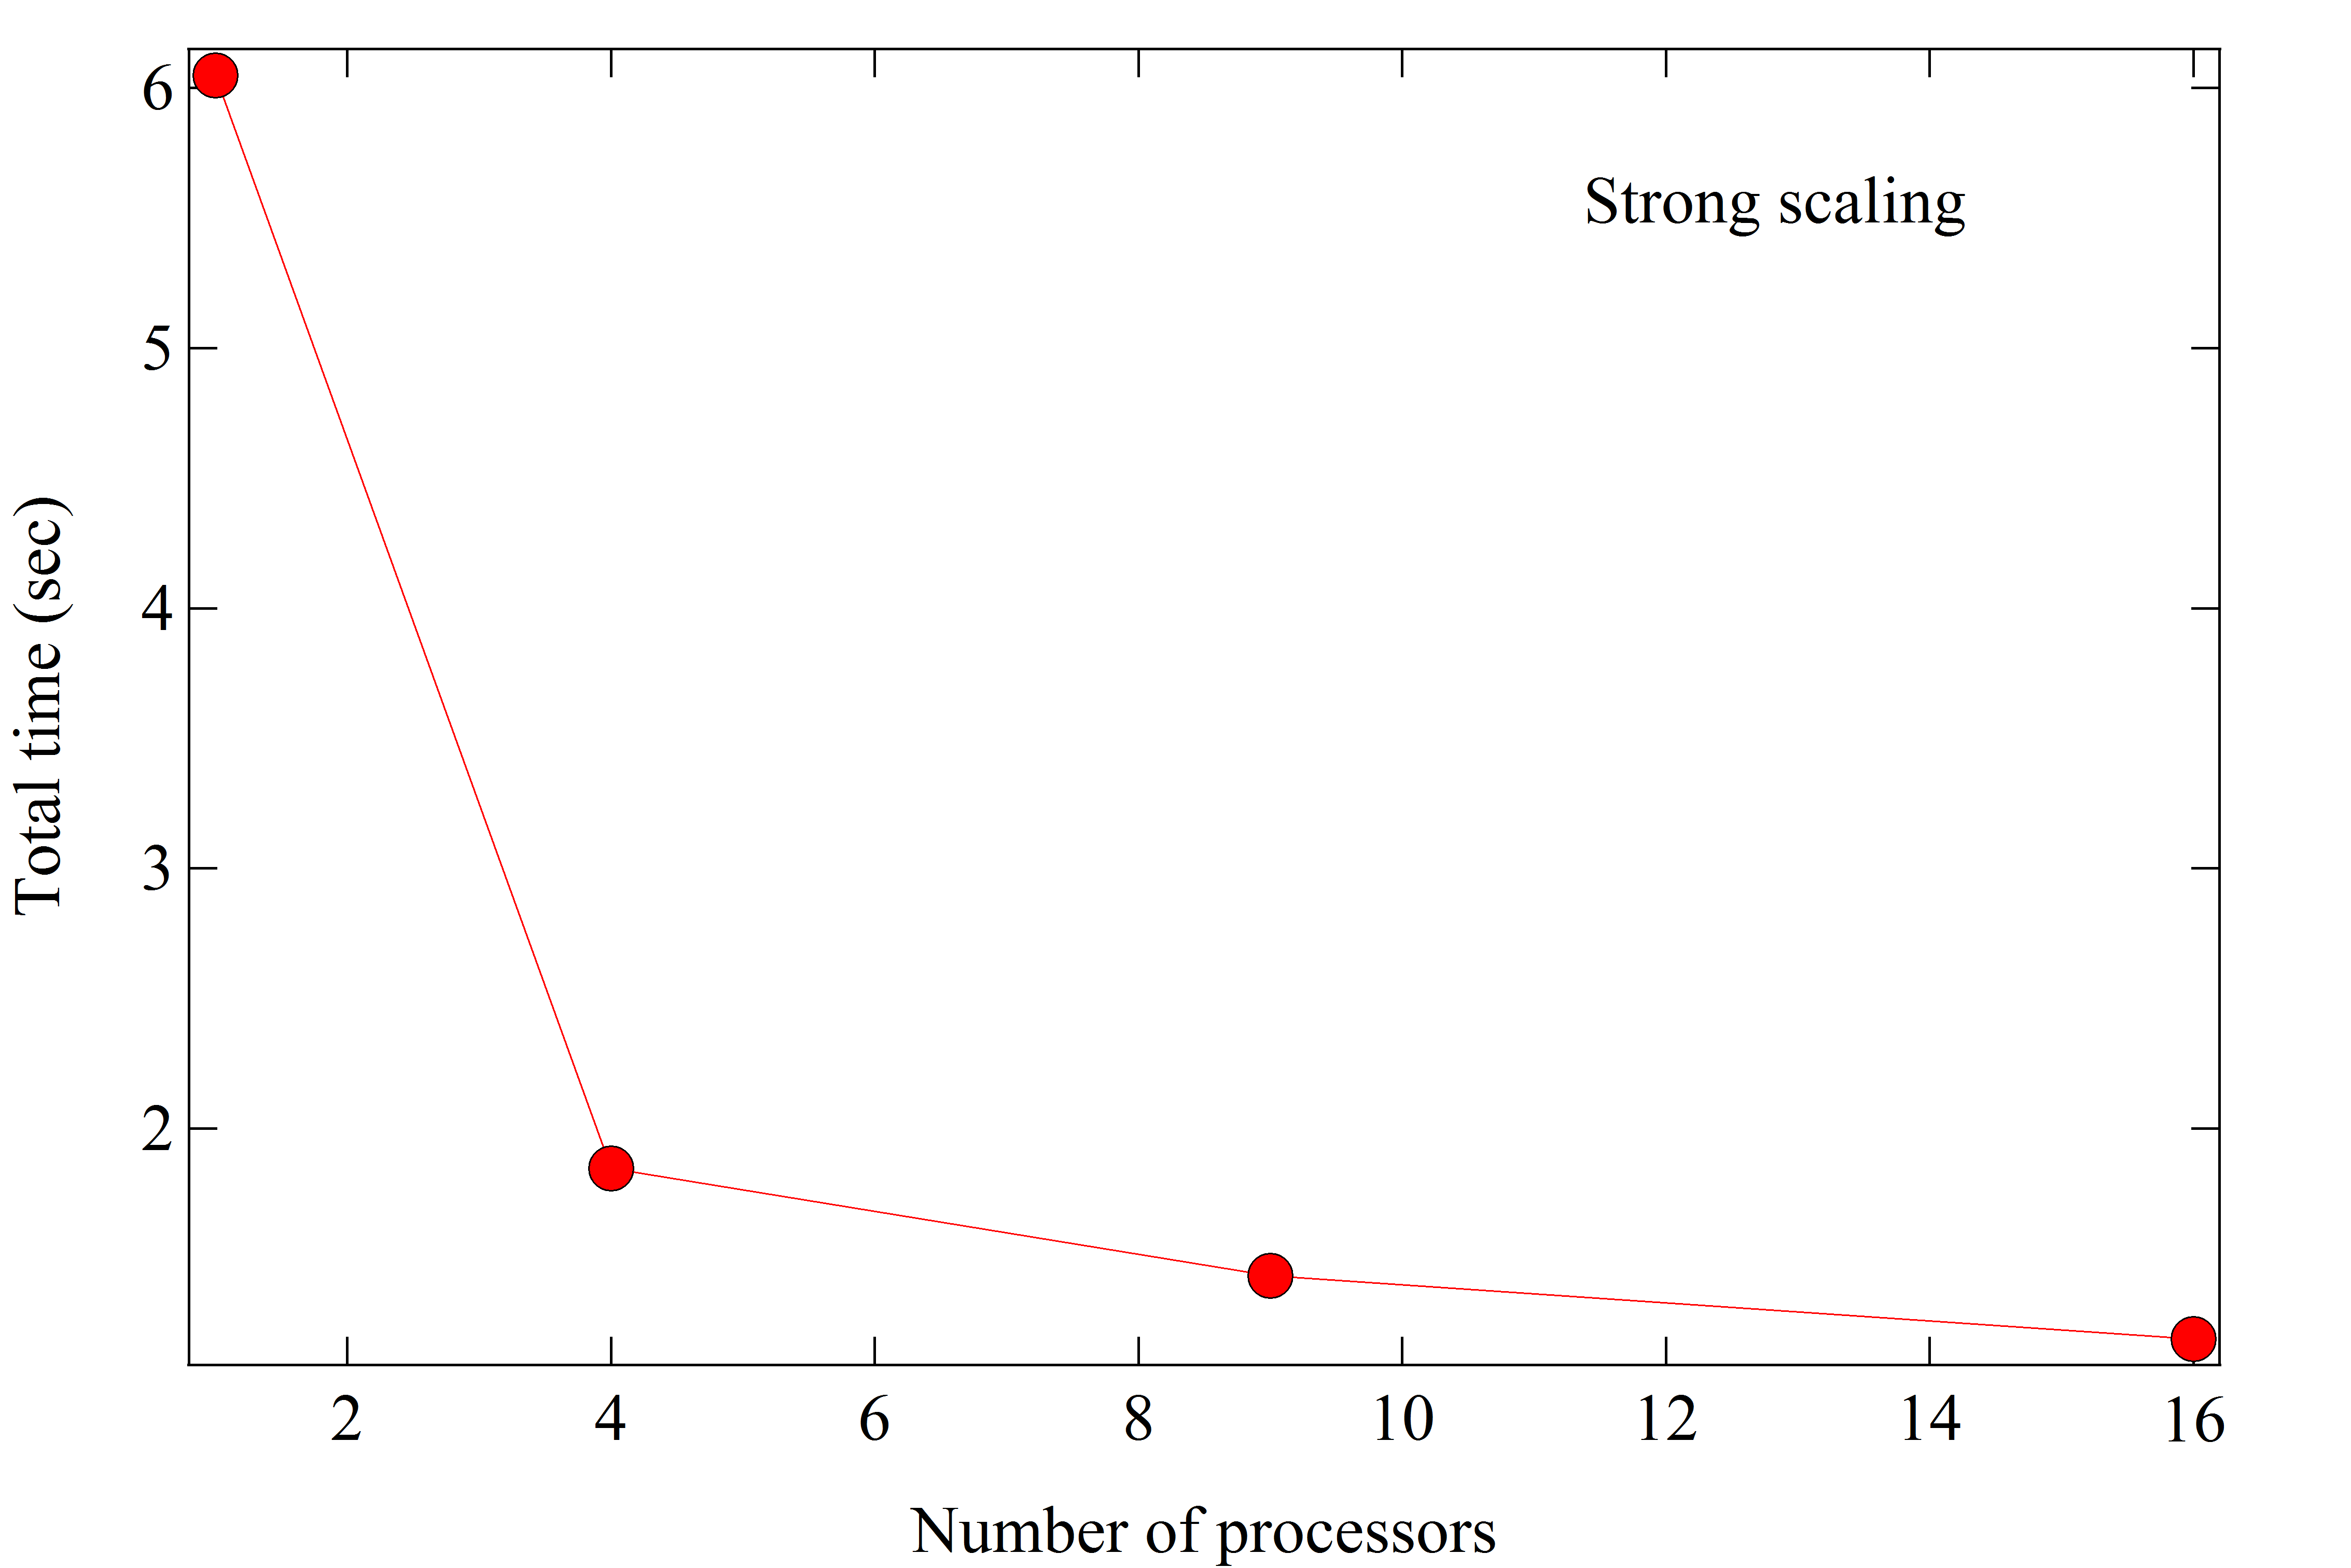
\includegraphics[width=5in]{strong.png}
        \end{figure}

        When performing these studies, we kept the number of frames constant at 50, and the size of the board constant at 300 $\times$ 300.

        When we look at the results, the total time taken decreases significantly decreases initially, but as we throw more and more processors at the problem, the speedup plateaus. This is most likely because with a fewer processors, there is little communication overhead. However, when we throw more processor at it, the communication overhead increases and as a result, the speedup is not as significant.

        One of the ways we could avoid this issue is to use \texttt{omp critical} or \texttt{omp atomic}. Another thing we could have done is to use two copies of the board. On even time steps we could then write to the first copy of the board and on odd timesteps, we could write the second copy of the board. As a result, we would only have one barrier instead of two, which would reduce the amount of time threads are idle and potentially increase speedup.

        According to Amdahl's law, the speedup we should see according to this simple model is:
        \begin{align*}
            S(p) \leq \frac{1}{\alpha + (1-\alpha)/p} \leq \frac{1}{\alpha}
        \end{align*}

        where $\alpha$ is the fraction of serial work that cannot be parallelized. Therefore, because there is some fraction of serial work that cannot be parallelized. Therefore, the amount of time that it takes for the simulation to run should approach the amount of serial work there is. If there were no serial work, then the speedup should be directly proportional to the number of processors.

        If we compare the parallelized code with the serial code, we see a total speedup of:
        \begin{align*}
            Speedup = \frac{6.0 \text{ seconds}}{1.2 \text{ seconds}} = 5
        \end{align*}

    \subsection{4.2 Weak Scaling}
        \begin{figure}[H]
            \centering
            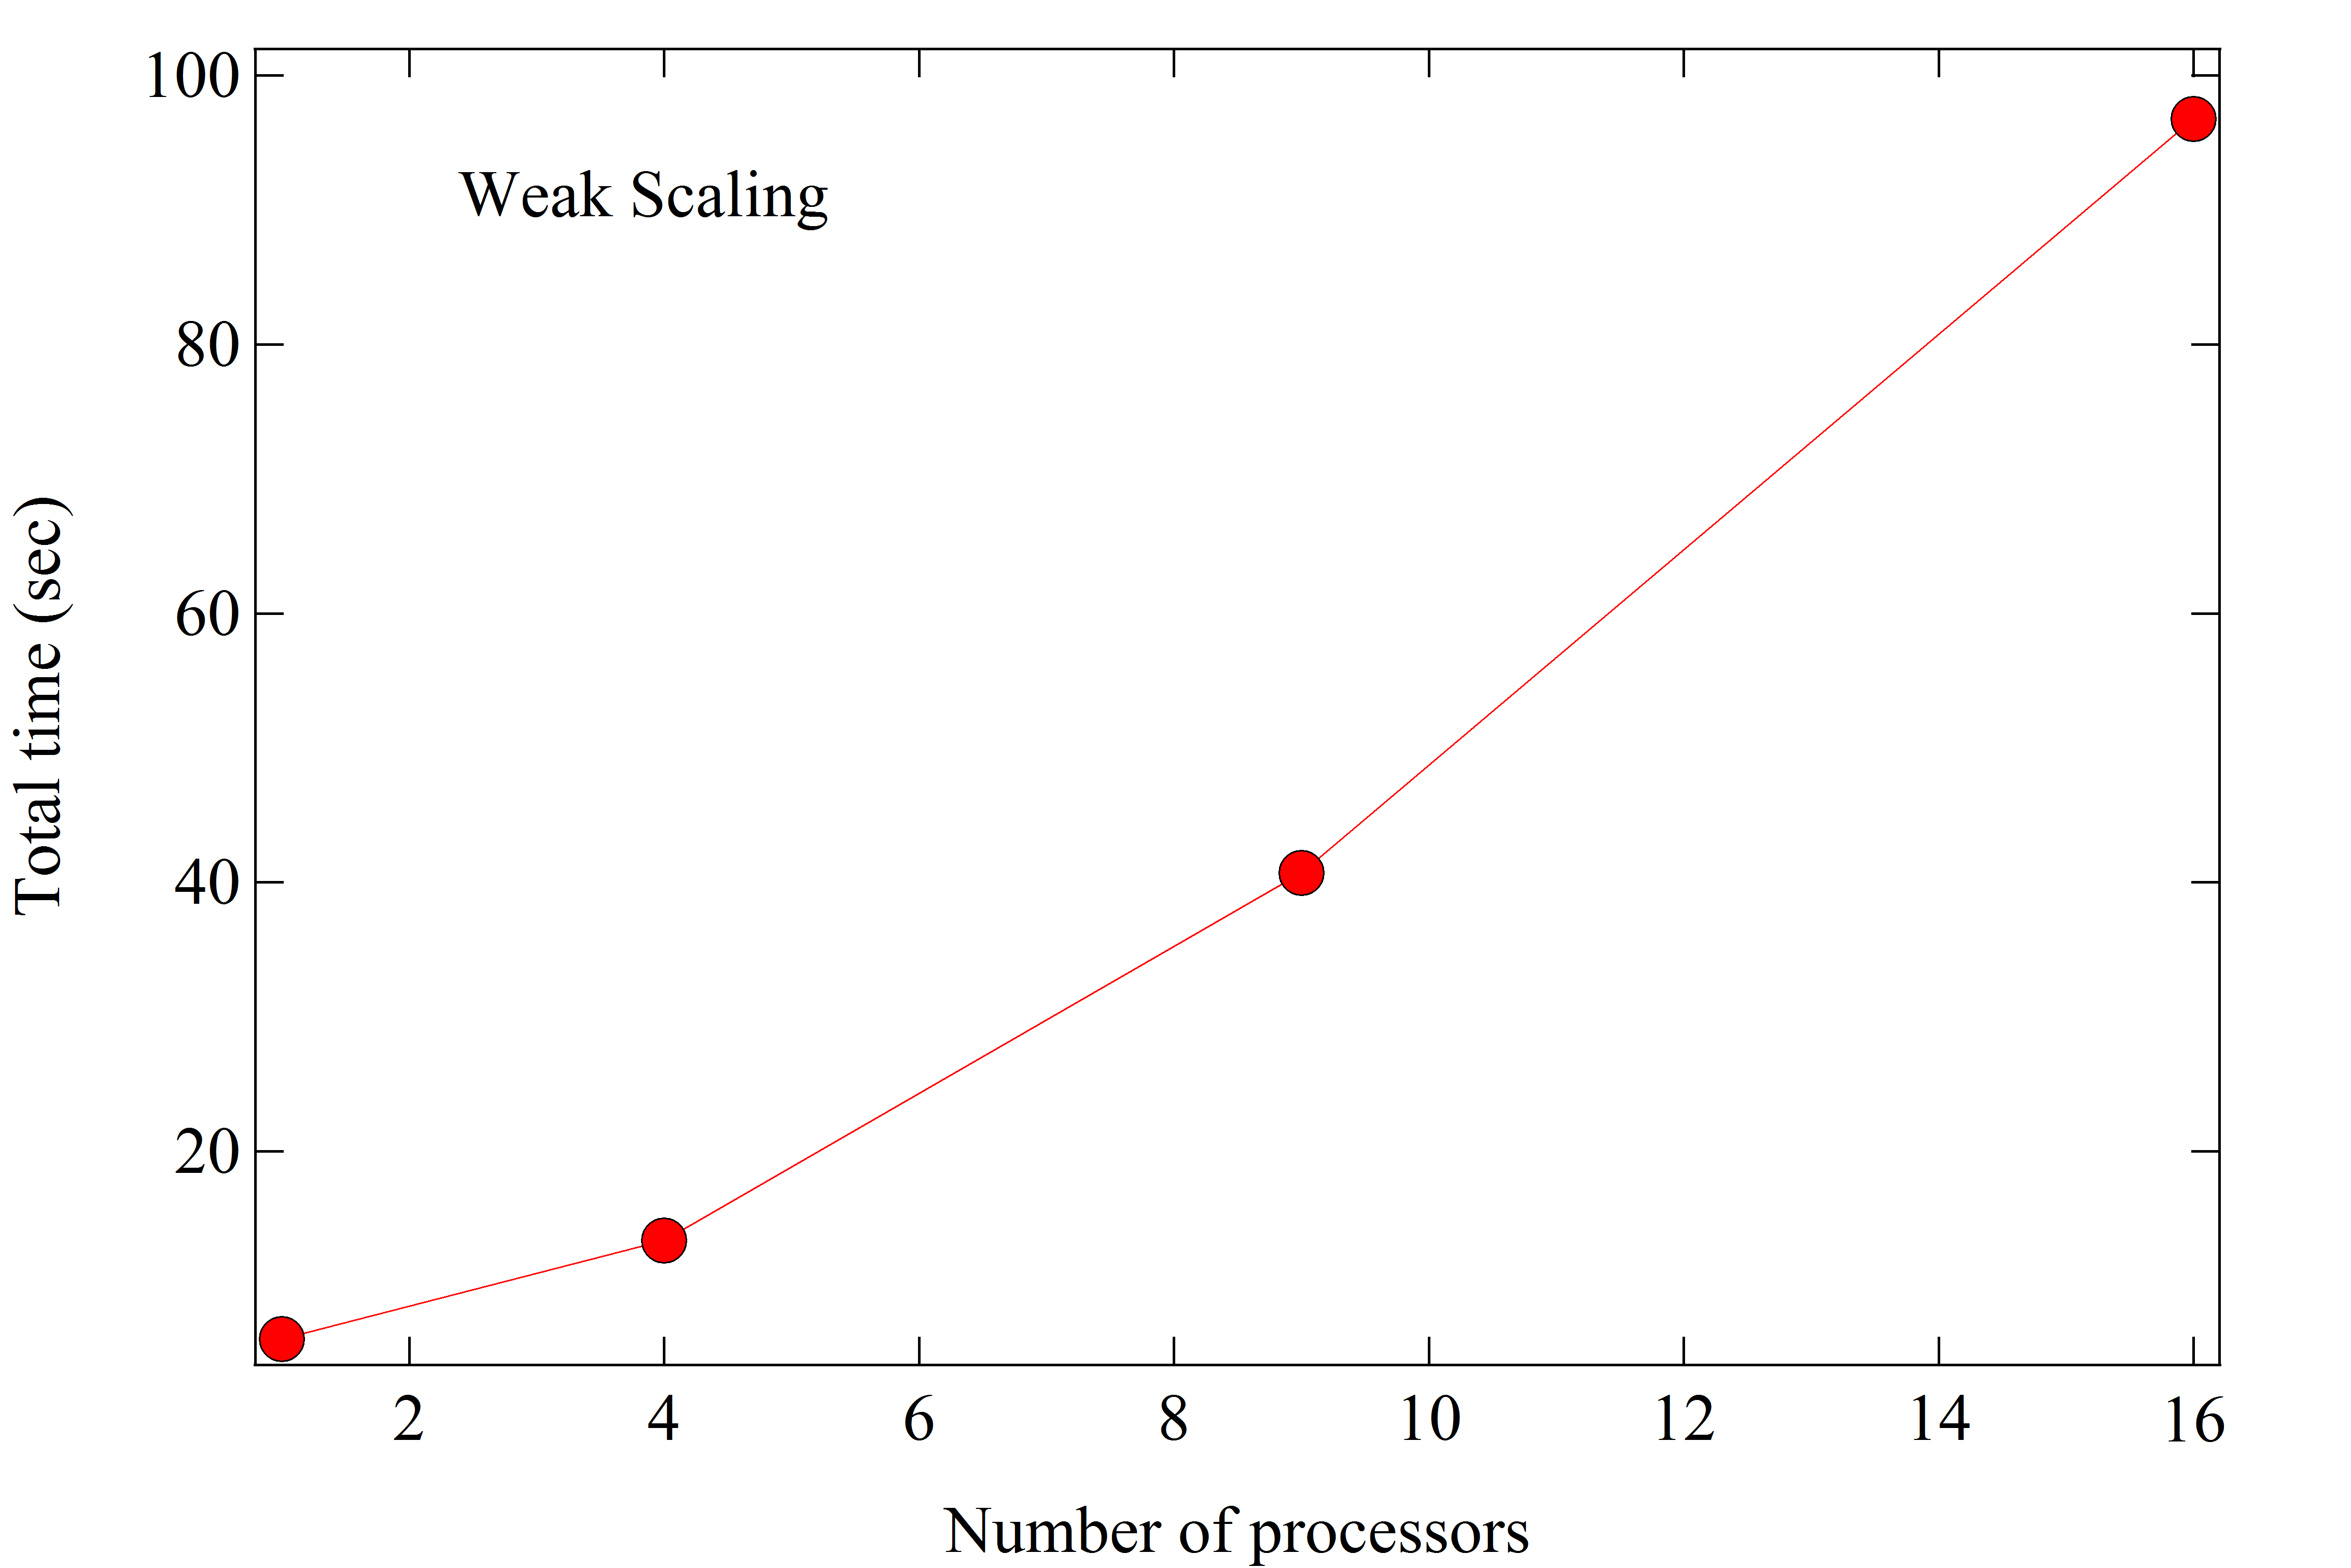
\includegraphics[width=5in]{weak.png}
        \end{figure}

        When performing these studies, we kept the number of frames constant, but we increased the size of the board proportional to the number of processors. The exact board sizes and number of threads we used were:

        \begin{figure}[H]
            \centering
            \begin{tabular}{c | c}
            Number of threads & Board size\\
            \hline
            1 & 300 x 300\\
            4 & 600 x 600\\
            9 & 900 x 900\\
            16 & 1200 x 1200
            \end{tabular}
        \end{figure}

        Ideally, if there were no serial overhead and no communication overhead, then the amount of time should be constant as we increase the size of the board proportional to the number of processors. However, this is not the case. The deviation from a constant time for increasing number of processors indicates that there is increasing communication overhead as we increase the number of processors and we are increasing the amount of serial work when we increase the number of processors. 
\end{document}